\section{Messdatenbilder}
\begin{figure}[htbp]            
\centering

\includegraphics[width=\textwidth]{assymetric_weakcoupling.pdf}
\caption{Asymetrische Schwingung bei schwacher Kopplung: Leichter Schwebungseffekt und Amplitudenabnahme durch Reibung erkennbar}
\label{fig:assymetricweakcoupling}
\end{figure}
\newpage
\section{Harmonische Oszillatoren}
\definecolor{lightgrey}{RGB}{237,237,237}
% \definecolor{resultsbackground}{RGB}{219,229,241}
\begin{tcolorbox}[enhanced, title = \(\sim\) Dimitrij Bathauer \protect\autocite{Dimitrij},attach boxed title to bottom right, width=0.8\textwidth,colframe=black,colback=lightgrey,watermark text=Harmonische Oszillatoren,watermark color=white,watermark zoom = 1]
    \enquote{Aber gut, mein Hohn wird der eigentlichen Relevanz des Versuchs wirklich nicht gerecht
    (nur ein bisschen vielleicht). Es ist kaum übertrieben zu sagen, dass die Welt gefühlt
    nur aus harmonischen und anharmonischen Oszillatoren aufgebaut ist. Du, ich, Jens
    Swagner, deine Mutter, you name it! Alles im Endeffekt (vereinfacht dargestellt)
    Oszillatoren!}
\end{tcolorbox}
\definecolor{alphacolor}{RGB}{101,133,160}
\definecolor{alphacolorupperback}{RGB}{165,161,167}
\definecolor{alphacolorlowerback}{RGB}{211,28,40}

\begin{tcolorbox}[skin=bicolor,title={But one question remains:\\Swagner ist ein HO, aber sein Alpha auch?\;\protect\autocite{alphastrahler}},width=0.8\textwidth,flush right,colframe=alphacolorupperback,colback=alphacolorlowerback,colbacktitle=alphacolor,halign=flush center]
    
\includegraphics[width=\linewidth]{alphastrahler1.png}
\end{tcolorbox}

Also ich habe viel zu viel Zeit damit verschwendet, mir die \href{https://mirror.rabisu.com/mirrors/CTAN/macros/latex/contrib/tcolorbox/tcolorbox.pdf}{Documentation} vom \tcboxverb[colback=blueurllink!40!white]{tcolorbox} package anzuschauen. Man kann damit unendlich viel rumspielen. Aber es sieht dann trotzdem nach 1980-Design aus rip.

\nocite{experienceorb}

\section{Code-Anhang}
Bei den Funktionen habe ich teilweise Dinge von verschiedenen Altprotokollen zusammengesucht, und auf meine Bedürfnisse umgeschrieben. Die konkreten Berechnung sind dann eigenständig.
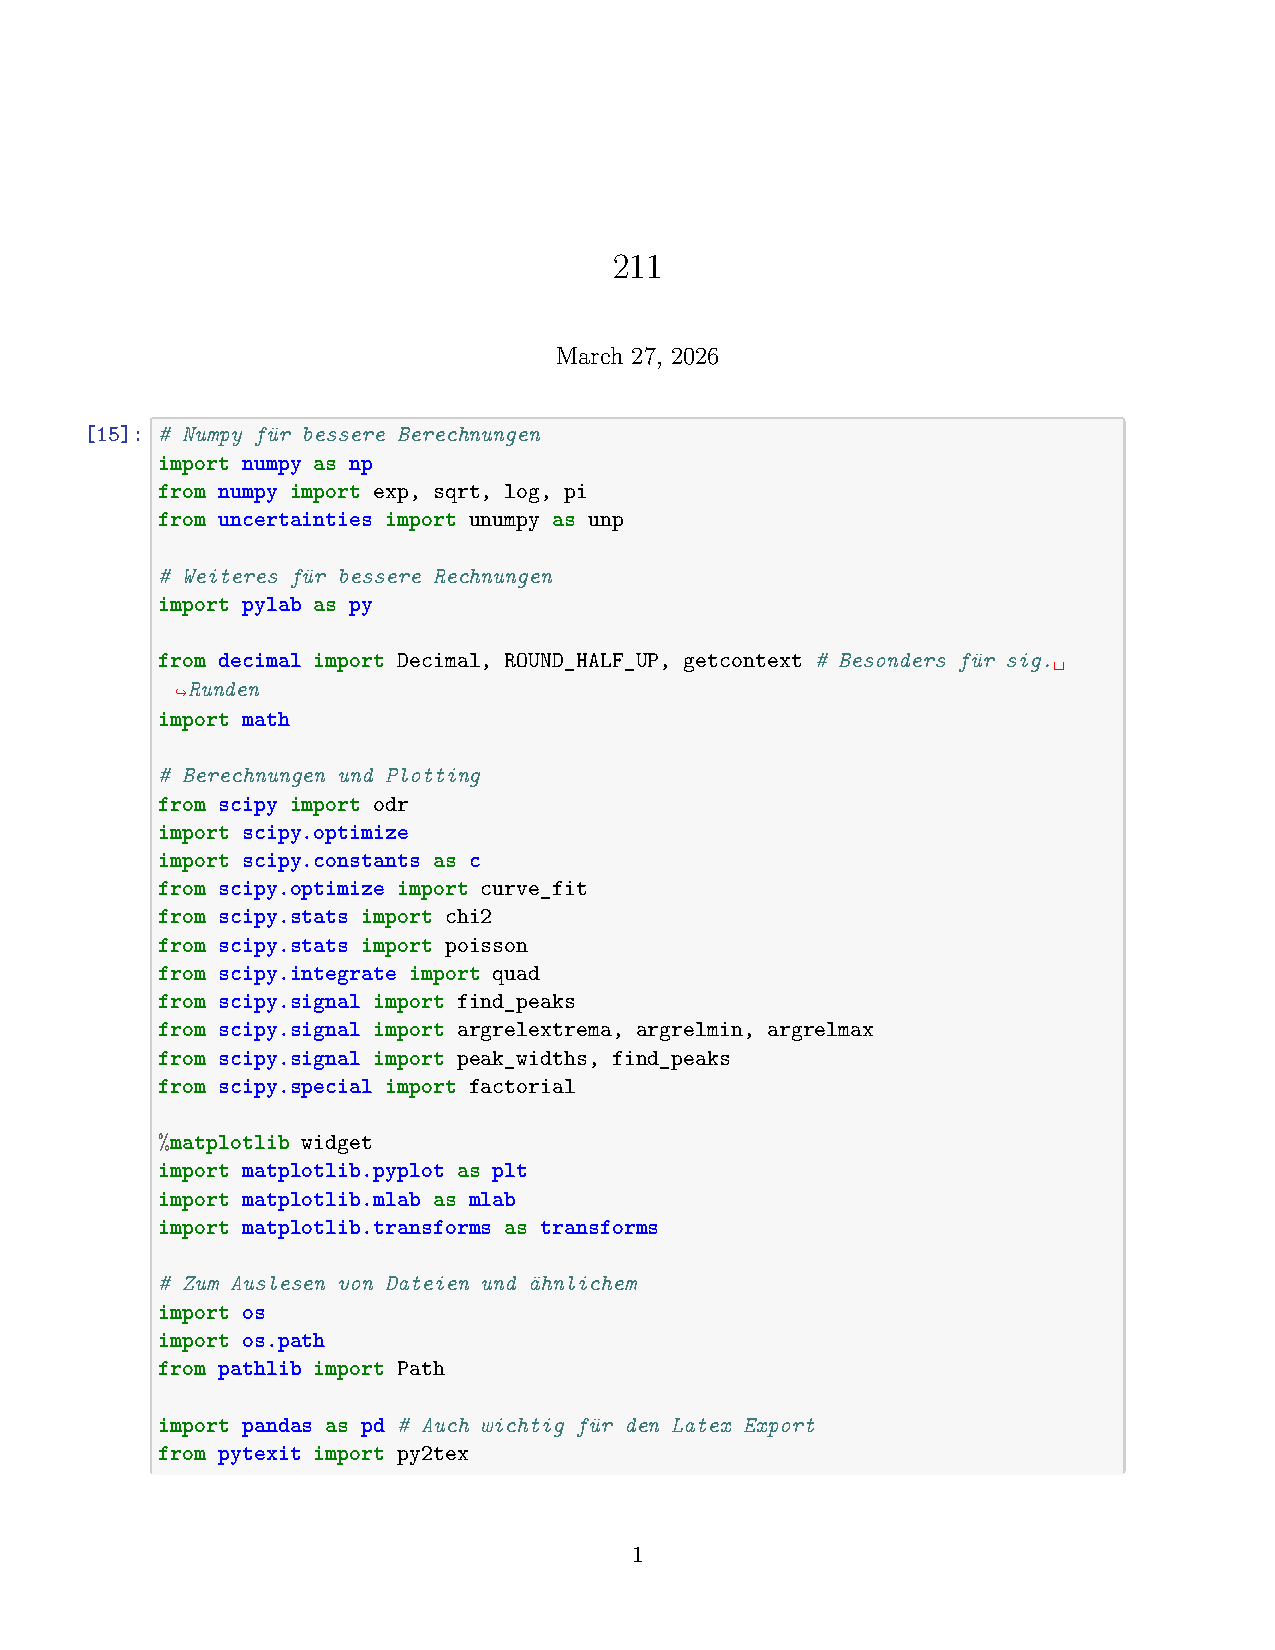
\includepdf[pages=-]{../Code/211/211.pdf}
